\documentclass[12pt, letterpaper]{article}
\usepackage[utf8]{inputenc}
\usepackage{setspace}
\usepackage{subcaption} 
\usepackage{hyperref}
\usepackage{float}
\usepackage{url}
\usepackage{amsthm}
\usepackage{graphicx}
\usepackage{amssymb}
\usepackage{amsmath}
\usepackage[lastexercise]{exercise}
\usepackage{tikz}
\usetikzlibrary{matrix}
\graphicspath{{images/}} \newtheorem{definition}{Definition}[section] \newtheorem{theorem}{Theorem}[section]
\newtheorem{corollary}{Corollary}[theorem]
\newtheorem{lemma}[theorem]{Lemma}
\newcommand{\R}{\mathbb{R}}
\newcommand{\Z}{\mathbb{Z}}
\newcommand{\implies}{\Rightarrow}
\title{Morse Theory}
\author{Veronika Starodub \\ Miloš Vukadinović \\ Nikolay Ninov} \date{\today } 
\doublespacing
\begin{document} 
\maketitle

\begin{figure}[h]
    \centering
    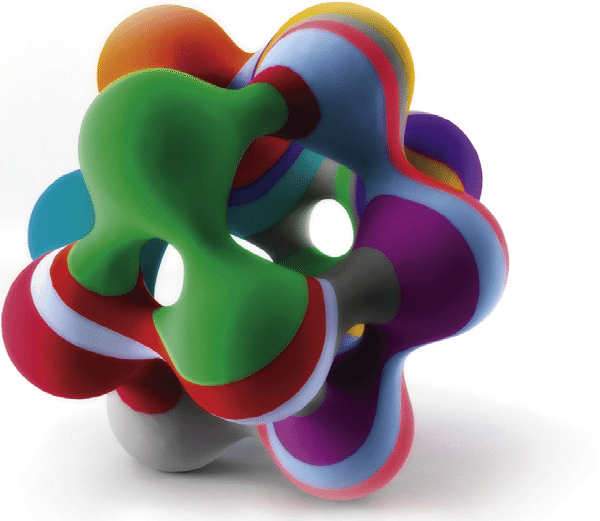
\includegraphics[width=0.50\textwidth]{cover}
\end{figure}
 
\tableofcontents
\section{Introduction}
\textbf{Ex.} Show that the function $f: S^2 \to \R, f(x,y,z) = z$ is a Morse function. \\

$f$ is smooth on $ S^2 $ since it extends to a smooth map on all of $\R^3$. We can map $R^3$ to $S^2$ with the stereographic projection two functions:\\
$
	\phi_1(x_1,x_2,x_3) = (\frac{x_1}{1-x_3}, \frac{x_2}{1-x_3} ) 
$
and
$
	\phi_2(y_1,y_2,y_3) = (\frac{y_1}{1+y_3},\frac{y_2}{1+y_3})
$\\
Therefore, to get $S^2 \to R^3$ we can take $\phi_1^{-1}$ and $\phi_2^{-1}$ \\
$
	\phi_1^{-1}(x_1,x_2,x_3) = (\frac{2x_1}{x_1^2+x_2^2+1}, \frac{2x_2}{x_1^2+x_2^2+1}, \frac{x_1^2+x_2^2-1}{x_1^2+x_2^2+1})
$\\
$
	\phi_1^{-1}(y_1,y_2,y_3) = (\frac{2y_1}{y_1^2+y_2^2+1}, \frac{2y_2}{y_1^2+y_2^2+1}, \frac{1-y_1^2+y_2^2}{y_1^2+y_2^2+1})
$\\
Then, we take $g_1 = f \circ \phi_1^{-1}$ and $g_2 = f \circ \phi_2^{-1}$ \\
$
	g_1(x,y) =  \frac{x^2+y^2-1}{x^2+y^2+1}
$
and
$
	g_2(x,y) = \frac{1-x^2+y^2}{x^2+y^2+1}
$ \\
Now, we can compute jacobian of $g_1$ and $g_2$, find critical points, and check that determinant of hessian matrix is non-zero. \\
$
	\nabla g_1(x,y,z) = 0$ iff $(x,y,z) = (0,0,-1)
$\\
$
	\nabla g_2(x,y,z) = 0$ iff $ (x,y,z) = (0,0,1)
$
We have two critical points, and now we compute the hessian at them.\\
$
	H(g_1) = \begin{bmatrix} 4 & 0 \\ 0 & 4 \end{bmatrix}
	\implies \det(H(g_1)) = 16
$\\
$
	H(g_2) = \begin{bmatrix} -4 & 0 \\ 0 & -4 \end{bmatrix}
	\implies \det(H(g_2)) =  16

$\\ 

Both critical points are non-degenerate, therefore $f$ is a Morse function.$\blacksquare$\\
\\
\\
Examples of Morse functions: \\
\textbf{Example 1.1}\\
$f(x,y)=e^{xy}+x$\\
First of all we have to find all critical points of $f$. A point $P$ is critical, when $\frac{\partial f}{\partial x}=\frac{\partial f}{\partial y}=0$ at $P$. \\
$\frac{\partial f}{\partial x}= ye^{xy}+1=0 \\
\frac{\partial f}{\partial y}=xe^{xy}=0$
After solving the system of equations we get that $x=0$, $y=-1$. Hence, the only critical point of $f$ is $(0,-1)$. Now to prove that the function is a Morse function we have to shoe that the determinant of Hessian matrix at the point $(0,-1)$ is non-zero. \\
Partial second order derivatives are: \\
$\frac{\partial^2 f}{\partial x^2}=y^2e^{xy}$
$\frac{\partial^2 f}{\partial x^2}(0,-1)=1$\\
$\frac{\partial^2 f}{\partial \partial y}=e^{xy}+yxe^{xy}$
$\frac{\partial^2 f}{\partial \partial y}(0,-1)=1$\\
$\frac{\partial^2 f}{\partial y \partial x}=e^{xy}+xye^{xy}$
$\frac{\partial^2 f}{\partial y \partial x}(0,-1)=1$\\
$\frac{\partial^2 f}{\partial y^2}=x^2e^{xy}$
$\frac{\partial^2 f}{\partial y^2}(0,-1)=0$\\
Therefore, \\
$det(Hess(f(0,-1)))=\left| \begin{array}{cc} 1 & 1 \\ 1 & 0 \end{array} \right|=-1$. \\
Since the determinant is non-zero at the only critical point of the function, we can claim that it is a Morse function. \\
\textbf{Example 1.2}\\
Let's consider a function $g(x,y)=xy$ and prove that it is , indeed, a Morse function.\\
First order partial derivatives: \\
$\frac{\partial g}{\partial x}=y$\\
$\frac{\partial g}{\partial y}=x$\\
Therefore, the only critical point of $g$ is $(0,0)$. Now we have to evaluate the determinant of Hessian matrix at this point.\\
Second order partial derivatives: \\
$\frac{\partial^2 g}{\partial x^2}=0$\\
$\frac{\partial^2 g}{\partial x \partial y}=1$\\
$\frac{\partial^2 g}{\partial y \partial x}=0$\\
$\frac{\partial^2 g}{\partial^2 y}=1$\\
Hence the determinant of Hessian at the critical point is: \\
$det(Hess(f(0,0)))=\left| \begin{array}{cc} 0 & 1 \\ 1 & 0 \end{array} \right|=-1$. \\
We observe that the determinant is nonzero, hence, the only critical point of $g(x,y)=xy$ is non-degenerate, so the function is Morse. \\
\\
\\
Examples of functions that are not Morse: \\
\textbf{Example 2.1}\\
$f(x,y)=x^3+xY^2-x^2y-y^3$\\
Let's follow the previous procedure: \\
$\frac{\partial f}{\partial x}=3x^2+y^2-2xy=0$\\
$\frac{\partial f}{\partial y}=2xy-x^2-3y^2=0$\\
After solving the system of equations we got that the only critical point of $f$ is $(0,0)$. Now compute second order partial derivatives:\\
$\frac{\partial^2 f}{\partial x^2}=6x-2y$\\
$\frac{\partial^2 f}{\partial x \partial y}=2y-2x$\\
$\frac{\partial^2 f}{\partial y \partial x}=2y-2x$\\
$\frac{\partial^2 f}{\partial^2 y}=2x-6y$\\
Therefore, \\
$det(Hess(f(0,0)))=\left| \begin{array}{cc} 0 & 0 \\ 0 & 0 \end{array} \right|=0$.\\
Hence, the only critical point of $f$ is degenerate, so $f$ is not a Morse function. \\
\textbf{Example 2.2}\\
$g(x,y)=x^3$\\
$\frac{\partial g}{\partial x}=3x^2$\\
$\frac{\partial g}{\partial y}=0$\\
Therefore, critical points are all points of the form $(0, y_1)$.\\
$\frac{\partial^2 g}{\partial x^2}=6x$
$\frac{\partial^2 g}{\partial x \partial y}=0$\\
$\frac{\partial^2 g}{\partial y \partial x}=0$
$\frac{\partial^2 g}{\partial^2 y}=0$\\
Hence, Hessian will be of the form: \\
$Hess(g(0,y_1))=\left| \begin{array}{cc} 0 & 0 \\ 0 & 0 \end{array} \right|,  \forall y_1$. \\
Therefore, all critical points of $g$ are degenerate points, moreover, values of $g$ at all critical points are equal, hence, $g(x,y)=x^3$ is not a Morse function. 


\end{document}
